% This file was created by matplotlib2tikz v0.7.4.
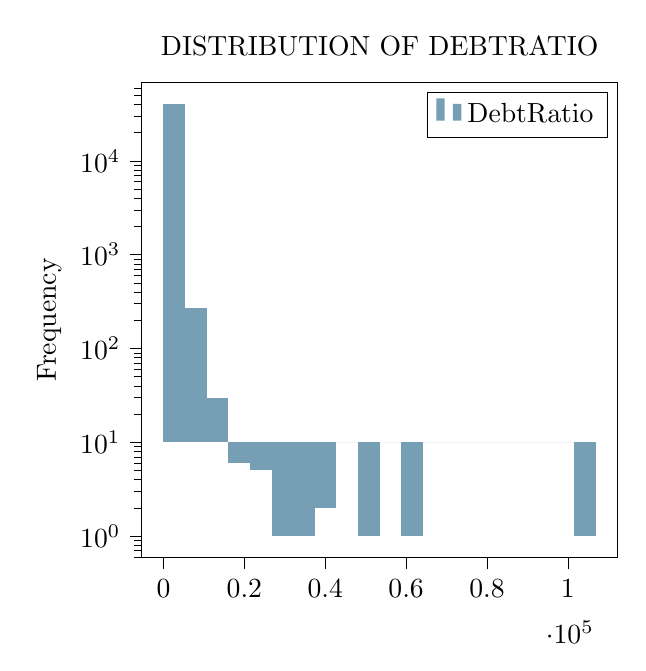
\begin{tikzpicture}

\definecolor{color0}{rgb}{0.462745098039216,0.623529411764706,0.713725490196078}

\begin{axis}[
height=3in,
log basis y={10},
tick align=outside,
tick pos=left,
title={\printsubsection{\MakeUppercase{Distribution of DebtRatio}}\\},
width=3in,
x grid style={white!69.01960784313725!black},
xmin=-5344.25, xmax=112229.25,
xtick style={color=black},
y grid style={white!69.01960784313725!black},
ylabel={Frequency},
ymin=0.588195747288335, ymax=69189.5515865574,
ymode=log,
ytick style={color=black}
]
\draw[fill=color0,draw opacity=0] (axis cs:0,0) rectangle (axis cs:5344.25,40697);
\addlegendimage{ybar,ybar legend,fill=color0,draw opacity=0};
\addlegendentry{DebtRatio}

\draw[fill=color0,draw opacity=0] (axis cs:5344.25,0) rectangle (axis cs:10688.5,271);
\draw[fill=color0,draw opacity=0] (axis cs:10688.5,0) rectangle (axis cs:16032.75,30);
\draw[fill=color0,draw opacity=0] (axis cs:16032.75,0) rectangle (axis cs:21377,6);
\draw[fill=color0,draw opacity=0] (axis cs:21377,0) rectangle (axis cs:26721.25,5);
\draw[fill=color0,draw opacity=0] (axis cs:26721.25,0) rectangle (axis cs:32065.5,1);
\draw[fill=color0,draw opacity=0] (axis cs:32065.5,0) rectangle (axis cs:37409.75,1);
\draw[fill=color0,draw opacity=0] (axis cs:37409.75,0) rectangle (axis cs:42754,2);
\draw[fill=color0,draw opacity=0] (axis cs:42754,0) rectangle (axis cs:48098.25,0);
\draw[fill=color0,draw opacity=0] (axis cs:48098.25,0) rectangle (axis cs:53442.5,1);
\draw[fill=color0,draw opacity=0] (axis cs:53442.5,0) rectangle (axis cs:58786.75,0);
\draw[fill=color0,draw opacity=0] (axis cs:58786.75,0) rectangle (axis cs:64131,1);
\draw[fill=color0,draw opacity=0] (axis cs:64131,0) rectangle (axis cs:69475.25,0);
\draw[fill=color0,draw opacity=0] (axis cs:69475.25,0) rectangle (axis cs:74819.5,0);
\draw[fill=color0,draw opacity=0] (axis cs:74819.5,0) rectangle (axis cs:80163.75,0);
\draw[fill=color0,draw opacity=0] (axis cs:80163.75,0) rectangle (axis cs:85508,0);
\draw[fill=color0,draw opacity=0] (axis cs:85508,0) rectangle (axis cs:90852.25,0);
\draw[fill=color0,draw opacity=0] (axis cs:90852.25,0) rectangle (axis cs:96196.5,0);
\draw[fill=color0,draw opacity=0] (axis cs:96196.5,0) rectangle (axis cs:101540.75,0);
\draw[fill=color0,draw opacity=0] (axis cs:101540.75,0) rectangle (axis cs:106885,1);
\end{axis}

\end{tikzpicture}